\subsection{Теоремы Кенига и тензор инерции}

\begin{definition}
    Система координат Кенига обладает следующими свойствами:
    \begin{enumerate}
        \item Имеет начало координат в центре масс.
        \item Движется поступательно относительно неподвижной системы координат, т.е. оси не меняют свою ориентацию.
    \end{enumerate}
\end{definition}
\begin{theorem}[Теорема Кенига о вычислении кинетической энергии]
    Кинетическая энергия механической системы представляется в виде суммы кинетической энергии центра масс системы и кинетической энергии относительного движения в осях Кенига:
    \[
    T = \dfrac{mv_C^2}{2} + T^\text{отн}
    \]
\end{theorem}

\begin{theorem}[Теорема Кенига о вычислении кинетического момента]
    Пусть задан полюс $B$. Тогда кинетический момент относительно него можно вычислить по формуле
    \[
    \vec{K}_B = \vec{K}_C +  m\vec{v}_C \times \vec{CB}
    \]
\end{theorem}
\begin{proof}
    В системе Кенига верно, что
    \[
    \vec{K}_C = \sum \vec{r}_{C_i} \times m\vec{v_i} = \sum \vec{r}_{C_i} \times m(\vec{v}_C +\vec{v}_i^{\text{отн}}) = \vec{K}_C^{\text{отн}}
    \]
    Пусть имеется два полюса: $A$ и $B$. Тогда получим формулу переноса полюса:
    \hypertarget{K_pole_shift}{}
    \[
    \begin{cases}
        \vec{K}_A = \sum \vec{r}_{A_i} \times m\vec{v_i}\\
        \vec{K}_B = \sum \vec{r}_{B_i} \times m\vec{v_i}\\
    \end{cases} \Longrightarrow \vec{K}_B = \vec{K}_A + \vec{p} \times \vec{AB}
    \]
    Подставив $A = C$, получим искомое.
\end{proof}

Аналогично для момента сил.\\

\hypertarget{tenzor}{}
Для любых двух векторов $\vec{a}$ и $\vec{b}$ векторное произведение можно задать через кососимметрический оператор:
\[
\vec{a} \times \vec{b} = \begin{pmatrix}
0 & -a_z & a_y\\
a_z & 0 & -a_x\\
-a_y & a_x & 0\\
\end{pmatrix} \cdot \vec{b}
\]

Тогда введем обозначение:
\[
R = \begin{pmatrix}
0 & -z & y\\
z & 0 & -x\\
-y & x & 0\\
\end{pmatrix}
\]
и заметим, что
\[
R^T \cdot R = \begin{pmatrix}
    y^2 + z^2 & -xy & -xz\\
    -xy & z^2 + x^2 & -yz\\
    -xz & -yz & x^2 + y^2\\
\end{pmatrix}
\]
--- это \textbf{тензор квадрата расстояния}, обозначается $j_{C_{xuz}}$. В физическом смысле тензор --- это признак сохранения/инвариантности и т.п. Например, масса является тензором.\\

Тогда кинетическая энергия твердого тела с неподвижной точкой (т.е. $\vec{v} = \vec{\omega}\times \vec{r}$):
\[
T = \dfrac{1}{2}\int \vec{v}^T \cdot \vec{v}dm = \dfrac{1}{2}\int (\vec{\omega} \times \vec{r})^T \cdot (\vec{\omega} \times \vec{r})dm = (*)
\]
Выразим векторное произведение через кососимметрический оператор: $\vec{\omega} \times \vec{r} = - R \cdot \vec{\omega}$. Тогда
\[
(*) = \dfrac{1}{3}\int (R \cdot \vec{\omega})^T \cdot (R \cdot \vec{\omega})dm = (*)
\]
Скалярное произведение инвариантно относительно замены базиса $\Longrightarrow$ перейдем в оси, жестко связанные с телом.
\[
(*) = \dfrac{1}{2}\int \vec{\omega}^T R^T\cdot R \vec{w} dm = \dfrac{1}{2}\vec{\omega}^TJ_{A_{xyz}}\vec{\omega}
\]

Здесь $J_{C_{xyz}} = \int R^T \cdot R ~dm$ --- \textbf{тензор инерции тела} относительно $C_{xyz}$. В осях, жестко связанных с телом, это неизменная характеристика тела.\\

Если есть тело и некоторая ось $\vec{e}$ в базисе, в котором посчитан тензор квадрата расстояний, то расстояние от точки до оси $d_C$ определяется как
\[
d_C^2 = \vec{e}^T j_{A_{xyz}}\vec{e}
\]

\begin{proposition}
    Для любых тел, полюсов и базисов всегда можно посчитать тензор инерции, т.е. он всегда существует.
\end{proposition}
\begin{proposition}
    Пусть 2 базиса с началом в точке О связаны ортогональной матрицей $S$: $\vec{r'} = S\vec{r}$. Тогда для тензоров верно
    \[
    {J'}_{A_{x'y'z'}} = S^T J_{A_{xyz}}S
    \]
\end{proposition}

\textbf{Момент инерции} твердого тела относительно некоторой оси $\vec{e}$
\[
J_{\vec{e}} = \int d_{\vec{e}}^2 dm = \vec{e}^T J_{A_{xyz}}\vec{e}
\]

Аналогично для кинетического момента  твердого тела с неподвижной точкой:
\[
\vec{K}_C = \int \vec{r}\times \vec{v}dm = \int R^T \cdot (-R\vec{\omega})dm = \int R^T \cdot R \vec{\omega} dm = J_{C_{xyz}} \vec{\omega}
\]

В плоском случае (считаем, что ось z ортогональна плоскости, в которой рассматривается движение тела):
\[
T = \dfrac{1}{2}J_z\omega^2 \ \text{и} \ \vec{K}_C = J_z \vec{\omega}
\]

\begin{example}
    \begin{figure}[!h]
        \centering
        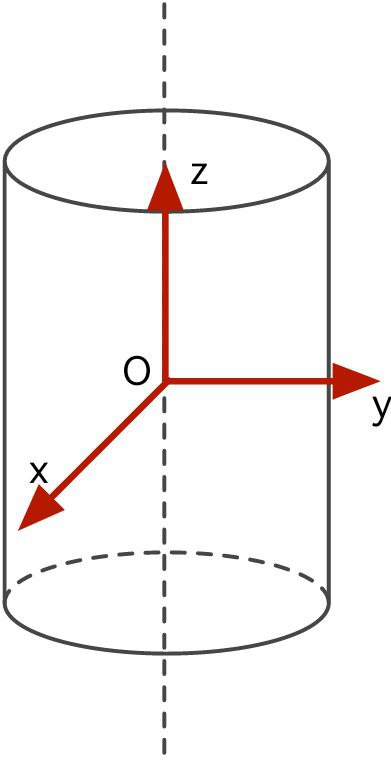
\includegraphics[width=0.2\linewidth]{images/лекция_6_1.jpeg}
    \end{figure}

    Вычислим тензор инерции $J_{O_{xyz}}$ сплошного однородного цилиндра массой $M$, радиусом $R$ и высотой $H$.\\

    \[
    J_{O_{xyz}} = \int \begin{pmatrix}
        y^2 + z^2 & -xy & -xz\\
    -xy & z^2 + x^2 & -yz\\
    -xz & -yz & x^2 + y^2\\
    \end{pmatrix}d m = \begin{pmatrix}
        A & -D & -E\\
        -D & B & -F\\
        -E & -F & C\\
    \end{pmatrix}
    \]
    Здесь $A$, $B$ и $C$ --- \textbf{осевые моменты инерции}; $D$, $E$ и $F$ --- \textbf{центробежные моменты инерции}. Из курса линейной алгебры известно, что любая симметрическая положительно определенная матрица может быть приведена к диагональному виду ($D$ = $E$ = $F$ = 0). Оси, в которых тензор инерции принимает такой вид, называются \textbf{главными осями инерции} тела, если оси еще и проходят через центр масс --- \textbf{центральными}.\\

    Перейдем к цилиндрическим координатам, в которых центробежные моменты равны нулю:
    \[
    \begin{cases}
        x = \rho \cos{\phi}\\
        y = \rho \sin{\phi}\\
        z = z\\
    \end{cases} \Longrightarrow \text{момент инерции относительно оси z:}
    \]
    \[
    C = \int (x^2 + y^2)d m = \dfrac{M}{\pi H R^2} \int \rho^2 \cdot \rho dV = \dfrac{M}{\pi H R^2} \int \limits_{-H/2}^{H/2}\int \limits_0^{2\pi} \int \limits_0^R \rho^3 ~d \rho ~d \phi ~d z = \dfrac{M}{\pi H R^2} \cdot \dfrac{R^4}{4} \cdot 2\pi \cdot H = \dfrac{MR^2}{2}
    \]
    Из симметрии $A = B$, тогда
    \[
    A + B = 2A = 2B = C + \int 2z^2 dm = C + \dfrac{2M}{\pi H R^2} \int \limits_{-H/2}^{H/2}\int \limits_0^{2\pi} \int \limits_0^Rz^2 \rho~d\rho~d\phi~d z = C + \dfrac{MH^2}{6} 
    \]
    \[
    \Longrightarrow \ A = B = \dfrac{MR^2}{4} + \dfrac{MH^2}{12}
    \]
\end{example}

Для реальных объектов вроде Земли и астероидов это не применимо. Формально, это даже не твердые тела.\\

Пусть $O$ --- произвольный полюс в твердом теле. Тогда элементарная работа сил над твердым телом:
\[
\delta A = \sum \vec{F}_i \vec{v}_i~ dt = (*)
\]
Т.к. тело твердое, а значит, расстояние между любыми двумя точками не меняется, $\vec{v}_i = \vec{v}_O + \vec{\omega}_O \times \vec{r}_{O_i}$. Тогда
\[
(*) = (\vec{R} \cdot \vec{v}_O)~d t + (\vec{M}_O \cdot \vec{\omega})~d t,
\]
где $\vec{F} = \sum \vec{F}_i$ --- \textbf{главный вектор системы сил}, а $\vec{M}_O$ --- \textbf{главный момент сил}.

\subsection{Основные теоремы динамики}
\begin{theorem}[Об изменении импульса]
\[
\dfrac{d \vec{P}}{d t} = \vec{F}^{out},
\]
где $\vec{P} = \sum m_i \vec{v_i}$.\\
Очевидно, что \textbf{закон сохранения импульса} --- частный случай этой теоремы.
\end{theorem}
\begin{note} $~$
    \begin{enumerate}
        \item Если нет внешних сил, то момент сохраняется.
        \item $m \vec{w}_c = \vec{F}^{out}$ --- \textbf{теорема о движении центра масс}
    \end{enumerate}
\end{note}

\begin{theorem}[Об изменении кинетического момента]
\hypertarget{theorem_delta_K}{}
    Пусть С --- центр масс тела, тогда кинетический момент относительно полюса А изменяется по закону
    \[
    \dfrac{d\vec{K_A}}{d t} = \vec{M_A^{out}} + m\vec{v_C} \times \vec{v_A}
    \]
\end{theorem}
\begin{proof}
    По определению момент импульса относительно $A$ $\vec{K_A} = \sum\limits_{i = 1}^{\infty} (\vec{r_i} - \vec{r_{A}}) \times m_i \ddot{\vec{r_i}}$. Тогда, учитывая, что
    \begin{itemize}
        \item импульс системы выражается через импульс центра масс;
        \item в ИСО второй закон Ньютона можно записать в виде $m_i\ddot{\vec{r_i}} = \vec{F}_i^{out} + \vec{F}_i^{in}$;
        \item $\sum \vec{F_i} = 0$, $\vec{M}_A^{in} = 0$, т.к. в силу третьего закона Ньютона внутренние силы компенсируют друг друга;
        
    \end{itemize}
    получим:
    \[
    \dfrac{d\vec{K_A}}{d t} = \dfrac{d}{d t} (\sum (\vec{r_i} - \vec{r_{A}}) \times m_i \ddot{\vec{r_i}}) = \sum (\vec{r_i} - \vec{r_{A}}) \times m_i \dot{\vec{v_i}} + \sum (\vec{v_i} - \vec{v_{A}}) \times m_i \vec{v_i} = \vec{M_A^{out}} + m\vec{v_C} \times \vec{v_A}
    \]
\end{proof}

Наиболее часто используются случаи, когда А является либо неподвижной точкой, либо центром масс. Тогда уравнение принимает вид
\[
\dfrac{d\vec{K_A}}{d t} = \vec{M_A^{out}}
\]

\begin{theorem}[Об изменении кинетической энергии]
    Изменение кинетической энергии зависит от внешних и внутренних сил следующим образом:
    \[
    \dfrac{d T}{d t} = N^{out} + N^{in},
    \]
    где $N^{out}$ --- мощность внешних сил, а $N^{in}$ --- внутренних.\\
    Или в дифференциальной форме:
    \[
    d T = \delta A^{out} + \delta A^{in},
    \]
    где $\delta A^{out}$ --- элементарная работа внешних сил, а $\delta A^{in}$ --- внутренних.
\end{theorem}
\begin{proof}
    Искомое утверждение получается дифференцированием кинетической энергии по времени с применением второго закона Ньютона:
    \[
    \dfrac{d T}{d t} = \sum m_i \ddot{\vec{r_i}} \vec{v_i} = \sum (\vec{F_i^{out}} + \vec{F_i^{in}}) \vec{v_i} = N^{out} + N^{in}
    \]
    Дифференциальная форма может быть получена из соотношения $\dfrac{d\vec{r_i}}{d t} = \vec{v_i}$.
\end{proof}


Напомним определение \hyperlink{def_potential_force}{потенциальной силы} в случае, уогда сила, действующая на точку зависит только от положения этой точки и времени. В случае, когда важно положение всех точек системы потенциальные силы определяются следующим способом.\\

\begin{definition}
    Силы $\vec{F_i} = \vec{F_i}(\vec{r}_1,~ ...,~ \vec{r_N},~t)$ называются \textbf{потенциальными}, если существует скалярная функция П$(\vec{r}_1,~ ...,~ \vec{r_N},~t)$ такая, что
    \[
    \vec{F}_i = - \dfrac{\partial \text{П}}{\partial \vec{r}_i}
    \]
    Здесь П --- \textbf{потенциальная энергия}.
\end{definition}

Отсюда получаем, что силы $\vec{F}_i$ потенциальны только тогда, когда выполнено
\[
\partial A = \sum \vec{F}_i \cdot d\vec{r_i} = -d \text{П} + \dfrac{\partial \text{П}}{\partial t}d t 
\]

Рассмотрим полную энергию $E = T + \text{П}$ в системе, в которой помимо непотенциальных, действуют потенциальные силы. Обозначим за $N^{\text{пот}}$ моощность потенциальных сил, а за $N^{\text{непот}}$ --- непотенциальных. Тогда из определения
\[
N^{\text{пот}} = - \sum \dfrac{\partial \text{П}}{\partial \vec{r_i}}\vec{r_i} = -\dot{\text{П}} + \dfrac{\partial\text{П}}{\partial t}
\]
Тогда дифференцируя $E$ по времени получим \textbf{закон изменения полной энергии}:
\[
\dfrac{d E}{d t} = N^{\text{непот}} + \dfrac{\partial \text{П}}{\partial t}
\]

Отсюда же получаем \textbf{закон сохранения энергии} в случае, когда силы консервативны и мощность непотенциальных сил равна нулю.\\